Wir betrachten als erstes Voronoi Kanten zwischen Punkt $P$ und Strecke $S$, diese bestehen Grundsätzlich aus 3 Abschnitten. (i) und (iii) sind Strecken bzw. Strahlen. Es ist die Voronoi Kante zwischen dem Punkt $P$ und dem linken $A$ bzw. rechten Streckenende $B$. (ii) ist eine Parabel, deren Form ist abhängig vom Abstand zwischen $P$ und $s$. In welchem Abschnitt $P$ liegt ist egal die Zusammensetzung der Voronoi Kante bleibt gleich.

\begin{figure}[h]
\begin{center}
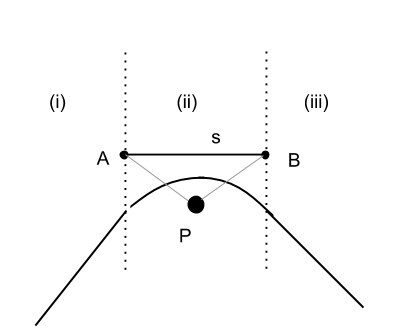
\includegraphics[width=7cm]{img/punkt-strecke.png}
\end{center}
\caption{Bisektor Punkt und Strecke}
\label{fig:c1}
\end{figure}


Betrachten wir nun die Bisektoren von zwei Strecken $s$ und $t$, dabei unterscheiden wir in (a) parallele Strecken und (b) nicht paralle Strecken.

zu (a): parallele Strecken:\\

(1) Strecken liegen auf einer Geraden\\
(2) überschneiden sich nicht\\
(3) überschneiden sich zum teil oder ganz\\

Hier entstehen jeweils 5 Bereiche, außer im Fall (1):\\
(i) Gerade: Bisektor von den linkesten Punkten $A$ und $C$\\
(ii) Parabel: $s$ und $C$\\
(iii) Gerade: Gerade dazwischen\\
(iv) Parabel: $t$ und $B$\\
(v) Gerade: Bisektor von den rechtesten Punkten $B$ und $D$\\

zu (b): nicht parallele Strecken:\\

(1) überschneiden sich nicht\\
(2) überschneiden sich zum teil oder ganz\\

Hier entstehen im Fall (1) 4 Bereiche, im Falls (2) 7 Bereiche:\\

wenn sie sich nicht überschneiden:\\
(i) Gerade\\
(ii) Winkelhalbierende\\
(iii) Parabel\\
(iv) Gerade\\

wenn sie sich überschneiden:\\
(i) Gerade\\
(ii) Parabel\\
(iii) Winkelhalbierende\\
(iv) Parabel\\
(v) Winkelhalbierende\\
(vi) Parabel\\
(vii) Gerade\\


* Wie sehen die Voronoi-Kanten aus $\rightarrow$ Bilder von allen Fällen\\
* Aus wie vielen Ecken, Kanten und Zellen kann $VD(S)$ höchstens bestehen?\\
* Zeigen Sie dazu, dass die Voronoi-Regionen zusammenhängend sind.